% Add example showing that if not SSA form, then could be many iterations for
% Cousot's operator.

% Add example showing that Cousot's does not reach fix-point always.

% Implement bck/RA8 and bck/RA9 to see how closer you get to the fix-point.

% Implement the fix point operator to solve the range analysis problem.

% How many instructions you cannot handle?

\documentclass[preprint]{sigplanconf}

\usepackage{amssymb}
\usepackage{amsmath}
\usepackage{graphicx}
\usepackage{skak} % for the \qside
\usepackage{mathpartir}
\usepackage{array}
\usepackage{url}

\newtheorem{theorem}{Theorem}[section]
\newtheorem{example}[theorem]{Example}
\newtheorem{lemma}[theorem]{Lemma}
\newtheorem{definition}[theorem]{Definition}

\newcommand{\fun}[1]{\mbox{\textbf{#1}}}
\newcommand{\lb}[1]{#1_{\downarrow}}
\newcommand{\ub}[1]{#1_{\uparrow}}
\newcommand{\varset}[1]{\mbox{$\cal{#1}$}}

\def\qed{\unskip\kern 10pt{\unitlength1pt\linethickness{.4pt}\framebox(6,6){}}}

\begin{document}

\conferenceinfo{Crazy Horse '11}{February 30th, 2011, Tumba, CA.} 
\copyrightyear{2011} 
\copyrightdata{[to be supplied]} 

\titlebanner{banner above paper title}
\preprintfooter{Range Analysis of Whole Programs}

\title{Range Analysis of Whole Programs}
\subtitle{}

\authorinfo{Homer Sympson \and Luck Skywalker \and Robin Hood \and
  Frodo Beggins}
           {Computer Science Department -- UFMG -- Brazil}
           {\{hsympson,skywalker,rbhood,frodo\}@dcc.ufmg.br}

\maketitle

\begin{abstract}
This paper describes a range analysis algorithm that is linear on the
program size.
We handle comparisons between variables via a two-phases dataflow analysis, and
achieve flow sensitiveness by using the Extended Static Single Assignment
form as the intermediate representation.
We have implemented an inter-procedural version of our technique into LLVM, an
industrial strenght compiler.
\end{abstract}

\category{D - Software}{D.3 Programming Languages}{D.3.4 Processors - Optimization}

\terms
Languages, Performance, Experimentation

\keywords
Range Analyisis, Dataflow Analysis, Integer arithmetics

\section{Introduction}
\label{sec:intro}

\section{Background}
\label{sec:bck}

% Define the lattice, the constraints and the valuation I.
Following Gawlitza {\em et al.}'s notation, we shall be performing arithmetic
operations over the complete lattice
$\cal{Z} = \mathbb{Z} \cup \{-\infty, +\infty\}$, where the ordering is
naturally given by $-\infty < \ldots < -2 < -1 < 0 < 1 < 2 < \ldots +\infty$.
For any $x > -\infty$ we define:

\begin{tabular}{lcl}
$x + \infty = \infty, x \neq -\infty$ & \mbox{\hspace{0.1cm}} & $x - \infty = - \infty, x \neq +\infty$ \\
$x \times \infty = \infty$ if $x > 0$ & & $x \times \infty = -\infty$ if $x < 0$ \\
$0 \times \infty = 0$ & & $(-\infty) \times \infty = \ $ not defined $$ \\
\end{tabular}

From the lattice $\varset{Z}$ we define the product lattice
$\varset{Z}^2$, which is partially ordered by the subset relation
$\sqsubseteq$.
$\varset{Z}^2$ is defined as follows:

\begin{equation*}
\varset{Z}^2 = \emptyset \cup \{[z_1, z_2] | \ z_1,z_2 \in \varset{Z},
\ z_1 \leq z_2, \  -\infty < z_2 \}
\end{equation*}

Given an interval $\iota = [l, u]$, we let $\lb{\iota} = l$, and
$\ub{\iota} = u$.
We let \varset{V} be a set of variables, and
$I: \varset{V} \mapsto \varset{Z}^2$ a
mapping from variables to intervals in $\varset{Z}^2$.
Our objective is to solve a constraint system $C$, formed by instances of the
five different types of constraints seen in Figure~\ref{fig:eval_function}
(left).
Figure~\ref{fig:eval_function} (right) defines a valuation function $e$ that
computes $Y = f(\ldots)$, given I.
Armed with these concepts, we define the range analysis problem as follows:

\begin{definition}
\label{def:rcp}
\textsc{Range Analysis Problem} \\
\textbf{Input:} a set $C$ of constraints ranging over a set \varset{V} of
variables. \\
\textbf{Output:} a mapping I such that, for any variable
$V \in \varset{V}$, e(V) = I[V].
\end{definition}

\begin{figure}[t!]
\begin{small}
\begin{eqnarray*}
\begin{array}{rc}
Y = [l, u]
&
e(Y) = [l, u]
\\
\\
Y = \phi (X_1, X_2)
&
\inferrule{I[X_1]=[l_1, u_1] \\ I[X_2]=[l_2, u_2]}
{e(Y) = [\mbox{min}(l_1, l_2), \mbox{max}(u_1, u_2)]}
\\
\\
Y = X_1 + X_2
&
\inferrule{I[X_1]=[l_1, u_1] \\ I[X_2]=[l_2, u_2]}
{e(Y) = [l_1 + l_2, u_1 + u_2]}
\\
\\
Y = X_1 \times X_2
&
\inferrule{I[X_1]=[l_1, u_1] \\ I[X_2]=[l_2, u_2] \\ L = \{l_1l_2, l_1u_2, u_1l_2, u_1u_2\}}
{e(Y) = [\mbox{min}(L), \mbox{max}(L)]}
\\
\\
Y = aX + b
&
\inferrule{I[X]=[l, u] \\ k_l = al + b \\ k_u = au + b}
{e(Y) = [\mbox{min}(k_l, k_u), \mbox{max}(k_l, k_u)]}
\\
\\
Y = X \sqcap [l', u']
&
\inferrule{I[X]=[l, u]}
{e(Y) \leftarrow [\mbox{max}(l, l'), \mbox{min}(u, u')]}
\end{array}
\end{eqnarray*}
\caption{\label{fig:eval_function}
The valuation function.}
\end{small}
\end{figure}

We will use the program in Figure~\ref{fig:ex1}(a) as the running example
to illustrate our range analysis.
Figure~\ref{fig:ex1}(b) shows the same program in SSA form, and
Figure~\ref{fig:ex1}(c) outlines the constraints that we extract from this
program.
There is a clear correspondence between instructions and constraints.
A possible solution to the range analysis problem is given in
Figure~\ref{fig:ex1}(d).
This is a very conservative solution.
As we will see shortly, we can improve this solution substantially by using
a more sophisticated program representation.

\begin{figure}[t!]
\begin{center}
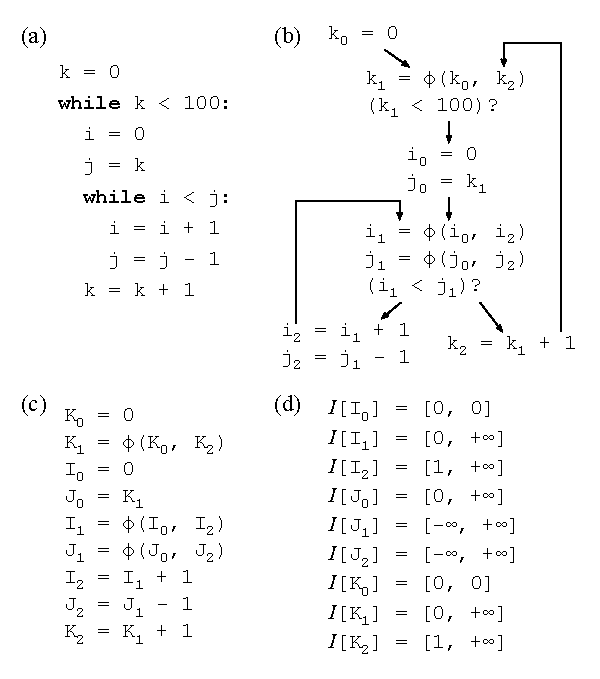
\includegraphics[width=\columnwidth]{images/ex1}
\end{center}
\caption{\label{fig:ex1}
(a) Example program.
(b) Control Flow Graph (CFG) in SSA form.
(c) Constraints that we extract from the program.
(d) A possible solution to the range analysis problem.}
\end{figure}


\section{Polynomial Time Range Analysis}
\label{sec:algo}

% Program representation
% Extracting constraints
% Building the Constraint graph (pseudo-edges)
% Macro algorithm
% Micro algorithm

In this section we explain the algorithm that we use to solve the range
analysis problem for an entire program.
This algorithm involves a number of steps.
First, we convert the program to a suitable intermediate representation that
makes it easier to extract constraint.
From these constraints, we build a dependence graph that allows us to do
range analysis sparsely.
Finally, we solve the constraints applying different fix-point iterators on
this dependence graph.
Figure~\ref{fig:algorithm} gives a global view of this algorithm.
Some of the steps in the algorithm are optional.
They improve the precision of the range analysis, at the expenses of a longer
running time.

\begin{figure}[t!]
\begin{center}
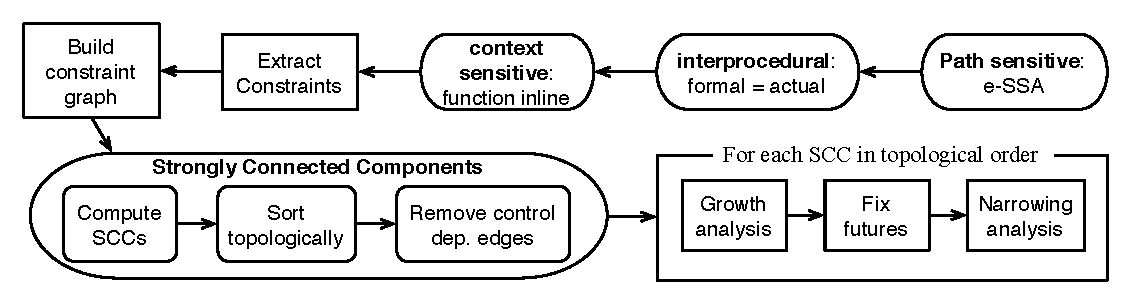
\includegraphics[width=\columnwidth]{images/algorithm}
\end{center}
\caption{\label{fig:algorithm}
Our algorithm to solve the range analysis problem.
Rounded boxes are optional steps.}
\end{figure}

\subsection{Choosing a Program Representation}
\label{sub:rep}

The solution that we found to the range analysis problem in Figure~\ref{fig:ex1}
is imprecise because we did not take conditional tests into considerations.
Branches gives us information about the ranges that some variables assume, but
only at {\em specific} program points.
For instance, given a test such as $(k_1 < 100)?$ in  Figure~\ref{fig:ex1}(b),
we know that $I[k_1] \sqsubseteq [-\infty, 99]$ whenever the condition is true.
In order to encode this information, we might split the live range of $k_1$
right after the branching point; thus, creating two new variables, one at the
path where the condition is true, and another where it is false.
There is a program representation, introduced by Bodik
{\em et al.}~\cite{Bodik00}, that performs this live range splitting:
the {\em Extended Static Single Assignment} form, or e-SSA for short.
In this paper, we have experimented with two different flavors of e-SSA form,
which we call {\em standard} and {\em non-pruned}.

We will show first how we convert a program into standard e-SSA form.
Let $(v < c)?$ be a conditional test, and let $l_t$ and $l_f$ be labels in
the program, such that $l_t$ is the target of the test if the condition is true,
and let $l_f$ is the target when the condition is false.
If $l_f$ dominates any use of $v$, then we insert at $l_f$ a copy
$v_f = v \sqcap [-\infty, c-1]$, where $v_f$ is a fresh name.
We then rename every use of $v$ that is dominated by $l_f$ to $v_f$.
Dually, if $l_t$ dominates any use of $v$, then we insert at $l_t$ a copy
$v_t = v \sqcap [c, +\infty]$, and rename variables accordingly.
If the test uses two variables, e.g., $(v_1 < v_2)?$, then we create
intersections bound to {\em futures}.
We insert, at $l_f$, $v_{1f} = v_1 \sqcap [\fun{ft}(v_2), +\infty]$,
and $v_{2f} = v_2 \sqcap [-\infty, \fun{ft}(v_1) - 1]$.
Similarly, at $l_v$ we insert
$v_{1v} = v_1 \sqcap [-\infty, \fun{ft}(v_2) - 1]$
and $v_{2f} = v_2 \sqcap [\fun{ft}(v_1), +\infty]$.
We use the notation $\fun{ft}(v)$ to denote the {\em future} bounds of a
variable.
As we will show in Section~\ref{sub:micro}, once the growth pattern of $v$ is
known, we can replace $\fun{ft}(v)$ by an actual value.
Once we are done placing copies, we insert $\phi$-functions into the
transformed program to convert it to SSA form.
This last step prevents that two different names given to the same original
variable be simultaneously alive at the program code.
Figure~\ref{fig:ex_standard_eSSA} shows our running example changed into
standard e-SSA form.

\begin{figure}[t!]
\begin{center}
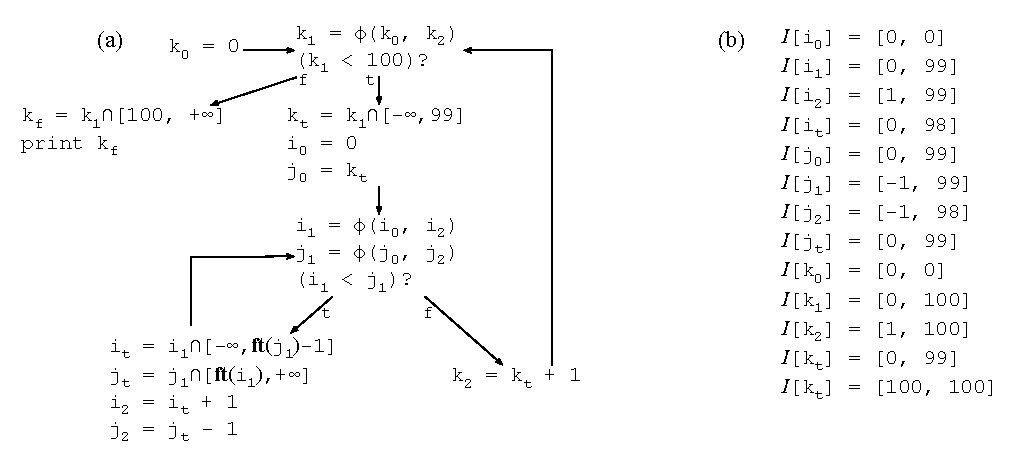
\includegraphics[width=0.7\columnwidth]{images/ex_standard_eSSA}
\end{center}
\caption{\label{fig:ex_standard_eSSA}
The control flow graph from Figure~\ref{fig:ex1}(b) converted to standard
e-SSA form.}
\end{figure}

The standard e-SSA form serves well analysis that need range information
at the use site of variables, such as conditional constant propagation,
redundant code elimination and detection of buffer overflows.
On the other hand, there exist compilation algorithms that require range
information at the whole live range of variables.
Examples of such algorithms include the family of
bitwidth aware register allocators~\cite{Barik06,Tallam03,Pereira08} and
hardware synthesizers~\cite{Cong05,Mahlke01,Stephenson00}.
In order to provide extra precision to these algorithms, we may work with a
non-pruned version of e-SSA form, which we produce by simply inserting copies
after every conditional test, and then reconverting the entire program to
SSA form.
Figure~\ref{fig:ex_non_pruned} illustrates the difference between these two
program representations.
Notice that the non-pruned flavor might introduce dead variables in the
program code, which can be removed by standard dead code elimination.

\begin{figure}[t!]
\begin{center}
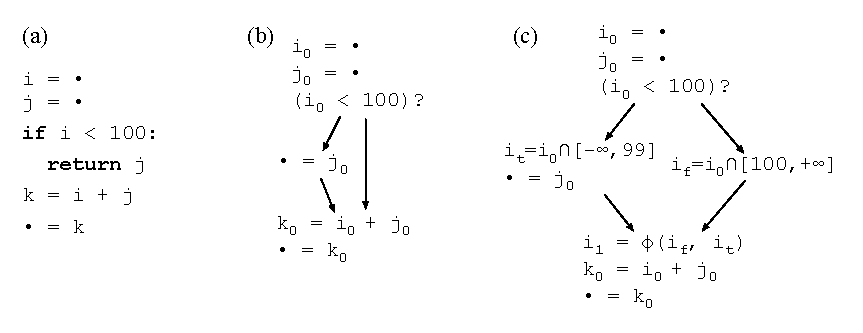
\includegraphics[width=\columnwidth]{images/ex_non_pruned}
\end{center}
\caption{\label{fig:ex_non_pruned}
(a) Example program.
(b) Standard e-SSA form.
(c) Non-pruned e-SSA form.}
\end{figure}

\subsection{Extracting Constraints}
\label{sub:constraints}

The constraints shown in Figure~\ref{fig:eval_function} let us handle
many different assembly instructions.
We use $\phi$ assignments, such as $Y = \phi(X_1, X_2)$ to represent
the $\phi$-functions typically found in SSA form programs.
As we have discussed in Section~\ref{sub:rep}, we use intersection
constraints to bound the variables created due to live range splitting
at conditionals.
The widening analysis that we will introduce in Section~\ref{sub:micro}
require monotonic transfer functions.
Many assembly operations, such as modulus or division, do not afford us
this property.
However, several of these non-monotonic instructions have a conservative
translation to our constraint system, as we show in
Figure~\ref{fig:constraints}.

\begin{figure}[t!]\begin{center}
\begin{tabular}{|l@{\hspace{0.2cm}}l@{\hspace{0.3cm}}l|} \hline
\textbf{Description} & \textbf{Operation} & \textbf{Constraint} \\ \hline
Constant & $v = c$ & $V = [c, c]$ \\
Assignment & $v_1 = v_2$ & $V_1 = V_2$ \\
Multiplication & $v_1 = v_2 * c$ & $V_1 = c V_2$ \\
Int. division & $v_1 = v_2 \ / \ v_3$ & $V_1 = V_2$ \\
 & & $V_1 = - V_2$ \\
Modulus & $v_1 = v_2 \ \% \ c$ & $V_1 = [0, c - 1]$ \\
Bitwise and & $v_1 = v_2 \ \& \ c$ & $V_1 = v_2 \sqcap [0, c]$ \\
Bitwise or & $v_1 = v_2 \ | \ v_3$ & $V_1 = V_2 + V_3$ \\
Left shift & $v_1 = v_2 \ \qside \ c$ & $V_1 = 2^c V_2$ \\ \hline
\end{tabular}
\end{center}
\caption{\label{fig:constraints}Example of constraint derivation rules.
We let $c$ denote a positive constant, $\{v, v_1, v_2\}$ are program
variables and $\{V, V_1, V_2\} \subset \cal{V}$.}
\end{figure}

\subsection{The Dependence Graph}
\label{sub:graph}

The main data structure that we use to solve the range analysis problem is
a variation of Ferrante {\em et al.}'s {\em program dependence
graph}~\cite{Ferrante87}.
For each constraint variable $V$ we create a variable node $N_v$.
For each constraint $C$ we create a constraint node $N_c$.
We add an edge from $N_v$ to $N_c$ if the name $V$ is used in $C$.
We add an edge from $N_c$ to $V$ if the constraint $C$ defines the name
$V$.
Figure~\ref{fig:ex_graph} shows the dependence graph that we build for the
e-SSA form program given in Figure~\ref{fig:ex_standard_eSSA}.
If $V$ is used by $C$ as the input of a future, then the edge from
$N_v$ to $N_c$ represents a {\em control
dependence}~\cite[p.323]{Ferrante87}.
All the other edges denote {\em data dependences}~\cite[p.322]{Ferrante87}.

\begin{figure}[t!]
\begin{center}
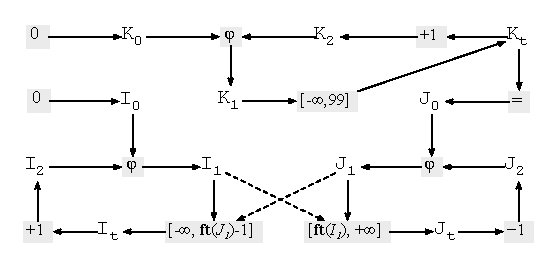
\includegraphics[width=\columnwidth]{images/ex_graph}
\end{center}
\caption{\label{fig:ex_graph}
The dependence graph that we build to the program in
Figure~\ref{fig:ex_standard_eSSA}.}
\end{figure}

\subsection{Finding Ranges: the Macro Algorithm}
\label{sub:macro}

Having built the dependence graph, we proceed to solve the range analysis
problem by finding all the strongly connected components (SCCs) of the
dependence graph, and reducing this graph to a directed acyclic graph.
We perform this last step by collapsing every SCC into a single node.
We then sort the resulting DAG topologically, and apply the analyses from
Section~\ref{sub:micro} on every SSC in topological order.
Once we solve the range analysis problem for a SCC, we propagate the
intervals that we found to the variable nodes at the {\em frontier} of this
SCC.
A variable node $N_v$ is said to be in the frontier of a strongly connected
component $S$ if:
(i) $N_v \notin S$; and
(ii) there exists a variable node $V' \in S$, and a constraint node $N_c$,
such that $V' \leftarrow N_c$, and $N_c \leftarrow V$.
This propagation gives us a very modular algorithm:
when analyzing a strongly connected component $S$ we can rest assured that
any influence that $S$ might suffer from nodes outside it has been already
taken into consideration.

\subsection{Finding Ranges: the Micro Algorithm}
\label{sub:micro}

Given a strongly connected component of the dependence graph with $N$ nodes,
we solve the range analysis problem in three-steps:
\begin{enumerate}
\item Run widening analysis: $O(N)$.

\item Fix intersections: $O(N)$.

\item Run narrowing analysis: $O(N^2)$.

\end{enumerate}
However, before we start, we remove the control dependence edges from the
strongly connected component, as they have no semantics to our transfer
functions.

\paragraph{Widening Analysis.}

The first step of our algorithm consists in determining the growth behavior of
the interval bound to each constraint variable.
We accomplish this task via Cousot and Cousot's widening
operator~\cite[p.247]{Cousot77}.
The possible behaviors of an interval are:
(i) does not change;
(ii) grows towards $+\infty$;
(iii) grows towards $-\infty$; and
(iv) grows in both directions.
The lattice of this dataflow analysis, plus its meet operator is given in
Figure~\ref{fig:growth_analysis}.
Because the lattice has height three, the intervals bound to each variable can
change at most three times.

\begin{figure}[t!]
\begin{tabular}{cc}
\begin{minipage}{2.4cm}
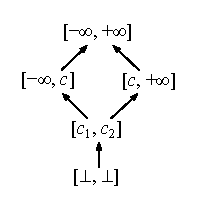
\includegraphics{images/growth_lattice}
\end{minipage}
&
\begin{minipage}{6cm}
\begin{small}
\begin{eqnarray*}
\begin{array}{c}
\inferrule{I[Y] = [\bot, \bot]}{I[Y] \leftarrow e(Y)}
\\
\\
\inferrule{\lb{e(Y)} < \lb{I[Y]} \\ \ub{e(Y)} > \ub{I[Y]}}
{I[Y] \leftarrow [-\infty, +\infty ]}
\\
\\
\inferrule{\lb{e(Y)} < \lb{I[Y]}}
{I[Y] \leftarrow [-\infty, \ub{I[Y]}]}
\\
\\
\inferrule{\ub{e(Y)} > \ub{I[Y]}}
{I[Y] \leftarrow [\lb{I[Y]}, +\infty]}
\end{array}
\end{eqnarray*}
\end{small}
\end{minipage}
\end{tabular}
\caption{\label{fig:growth_analysis}
(Left) The lattice of the widening analysis.
(Right) Cousot and Cousot's widening operator. We evaluate the rules from top 
to bottom, and stop upon finding a pattern matching.}
\end{figure}

\paragraph{Fixing futures.}

The ranges found by the widening analysis tells us which variables have fixed
bounds, independent on the intersections in the constraint system.
Thus, we can use actual limits to replace intersections bounded by futures.
Figure~\ref{fig:fix_intersects} shows the rules to perform these substitutions.
In order to correctly replace a future $\fun{ft}(V)$ that limits a variable
$V'$, we need to have already applied the widening analysis onto $V$.
Had we considered only data dependence edges, then it would be possible
that $V$ be analyzed before $V'$.
However, because of control dependence edges, this case cannot happen.
The control dependence edges ensure that any topological ordering of the
constraint graph either places $N_v$ before $N_{v'}$, or places these nodes
in the same strongly connected component.
For instance, in Figure~\ref{fig:ex_graph}, variables $J_1$ and $I_t$ are in
the same SCC only because of the control dependence edges.

\begin{figure}[t!]
\begin{center}
\begin{eqnarray*}
\begin{array}{c}
\inferrule{Y = X \sqcap [l, \fun{ft}(V) + c] \\ \ub{I[V]} = u}
{Y = X \sqcap [l, u + c]}, u, c \in \mathbb{Z} \cup \{-\infty, +\infty\}
\\
\\
\inferrule{Y = X \sqcap [\fun{ft}(V) + c, u] \\ \lb{I[V]} = l}
{Y = X \sqcap [l + c, u]}, l, c \in \mathbb{Z} \cup \{-\infty, +\infty\}
\end{array}
\end{eqnarray*}
\end{center}
\caption{\label{fig:fix_intersects}Rules to replace futures by actual
bounds. $S$ is the interval bound to each variable after the widening
analysis.}
\end{figure}

%\begin{figure}[t!]
%\begin{equation*}
%S[X] \leftarrow
%\begin{cases}
%``\ ? \ " \ \ \mbox{if} \ I[X] = [-\infty, +\infty]\\
%``\downarrow" \ \mbox{if} \ I[X] = [-\infty, c], c \in \mathbb{Z} \\
%``\uparrow" \ \mbox{if} \ I[X] = [c, +\infty],  c \in \mathbb{Z} \\
%`` \ 0 \ " \ \ \mbox{if} \ I[X] = [c_1, c_2], c_1, c_2 \in \mathbb{Z}
%\end{cases}
%\end{equation*}
%\caption{\label{fig:st_mem}The growth state of each variable.}
%\end{figure}

\paragraph{Narrowing Analysis.}

The widening analysis associates very conservative bounds to each variable.
Thus, the last step of our algorithm consists in narrowing these intervals.
We accomplish this step via Cousot and Cousot's narrowing
operator~\cite[248]{Cousot77}, which we show in
Figure~\ref{fig:crop_analysis}.

\begin{figure}[t!]
\begin{center}
\begin{eqnarray*}
\begin{array}{c}
\inferrule{\lb{I[Y]} = -\infty \\ \lb{e(Y)} > -\infty}
{I[Y] \leftarrow [\lb{e(Y)}, \ub{I[Y]}]}
\\
\\
\inferrule{\lb{I[Y]} > \lb{e(Y)}}
{I[Y] \leftarrow [\lb{e(Y)}, \ub{I[Y]}]}
\\
\\
\inferrule{\ub{I[Y]} = +\infty \\ \ub{e(Y)} < +\infty}
{I[Y] \leftarrow [\lb{I[Y]}, \ub{e(Y)}]}
\\
\\
\inferrule{\ub{I[Y]} < \ub{e(Y)}}
{I[Y] \leftarrow [\lb{I[Y]}, \ub{e(Y)}]}
\end{array}
\end{eqnarray*}
\end{center}
\caption{\label{fig:crop_analysis}Cousot and Cousot's narrowing operator.}
\end{figure}

\paragraph{Example}

Continuing with our example, Figure~\ref{fig:ex_partition_grow_crop} shows
the application of our algorithm on the last strongly connected component of
Figure~\ref{fig:ex_graph}.
Notice that upon meeting this SCC, we have already found the interval
$[0, 0]$ to $I_0$ and the interval $[100, 100]$ to $J_0$, as we show in
Figure~\ref{fig:ex_graph}(a).
We are not guaranteed to find the least fix point of a constraint system.
However, in this example we did it.
We emphasize that finding this tight solution was only possible because of
the topological ordering of the constraint graph in
Figure~\ref{fig:ex_graph}.
Had we applied the widening operator onto the whole graph, then we would
have found out that variable $J_0$ is bound to $[-\infty, +\infty]$,
because
(i) it receives its interval directly from variable $K_t$, which is upper
bounded by $+\infty$, and
(ii) it is part of a negative cycle.
On the other hand, because we only analyze the $J$'s SCC after we have
analyzed $K$'s, $K$ only contribute the constant range $[0, 99]$ to $J_0$.


\begin{figure}[t!]
\begin{center}
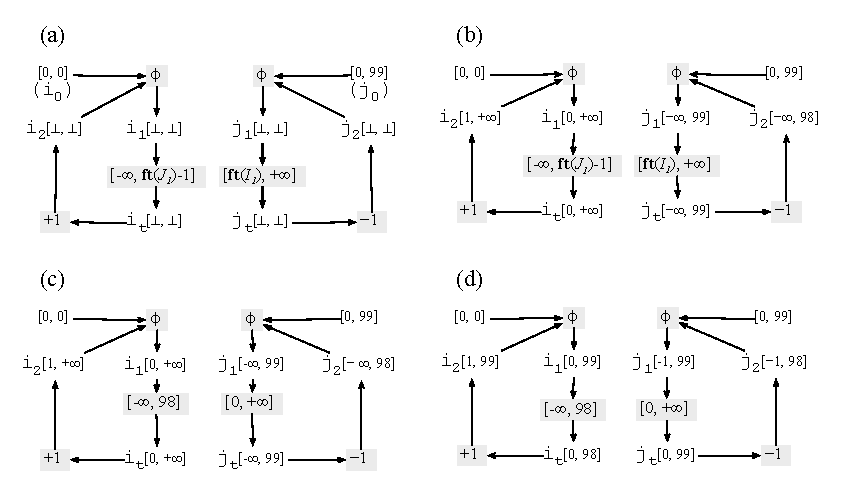
\includegraphics[width=\columnwidth]{images/ex_partition_grow_crop}
\end{center}
\caption{\label{fig:ex_partition_grow_crop}
Four snapshots of the last SCC of Figure~\ref{fig:ex_partition_grow_crop}.
(a) After removing control dependence edges, immediately before applying
Cousot and Cousot's operators.
(b) After running the widening analysis.
(c) After fixing the intersections.
(d) After running the narrowing analysis.}
\end{figure}

\subsection{Alternative Narrowing Operators}
\label{sub:alt}

Cousot and Cousot's narrowing operator, given in
Figure~\ref{fig:crop_analysis} is not guaranteed to find the least fixpoint
of a system of constraints.
In order to improve the bounds, trading time for precision, we have
experimented with two other operators.
The first, is the evaluation function itself, which is given in
Figure~\ref{fig:eval_function}.
By iterating it until reaching a fixpoint, we are guaranteed to find the
optimal solution to the narrowing analysis.
However, this approach is not practical, because it is equivalent to
concretely interpreting the program.
The second alternative that we have tested consists in applying the
evaluation function on each constraint at most once per intersection.
We call this approach {\em depth-first narrowing}, because, starting from
an intersection we visit every node that might be influenced by it.
After removing control dependence edges, if we are left with a strongly
connected component containing only {\em ascencing constraints}, that
is, constraints that only increase the upper bounds of intervals, then this
approach is guaranteed to find the least fixpoint.
The same is true if we have a SCC with only {\em descending constraints}.

\bibliographystyle{plain}
\bibliography{references}

\end{document}
